\documentclass[a4paper,12pt]{report}

\usepackage{prettylatex}
\usepackage{titlepage}
\usepackage{boiboites}
\usepackage{pgfplots}

\top{Université de Technologie de Belfort-Montbéliard}{}
\title{Cours d'IN41}{Analyse et traitement du signal}
\author{}
\date{Semestre de printemps 2016}

\newboxedtheorem[boxcolor=orange, background={rgb:white,20;green,2;black,1}, titlebackground={rgb:white,15;green,5;black,3},
titleboxcolor = black]{defi}{Définition}{cmpDefi}

\begin{document}

\maketitlepage

\tableofcontents
\pagebreak

\chapter{Représentation et classification des signaux}

\begin{defi}[Signal]
    Un signal est une information relative à une grandeur physique qui évolue dans le temps. C'est une fonction définie telle que :
    \begin{align*}
        S : E & \to \mathbb{R} & \text{ avec } E \subset \mathbb{R} \\
        t & \longmapsto S(t) &
    \end{align*}
\end{defi}

\neverindent

\section{Types de signaux}

Signal analogique : si $E$ est un intervalle réel $\implies$ signal analogique ou continu. \\
Signal numérique : si $E = \mathbb{Z} \implies$ signal discret ou numérique. \\
Signal échantillonné : si $E = \{t_{1}, t_{2}, ..., t_{n}\} \implies$ signal échantillonné.

\section{Analyse et reconstitution des signaux}

\textbf{\'Etape 1} : Reconstituer un signal : déterminer le signal $s$ à partir de la superposition des fonctions élémentaires données pour obtenir une synthèse. \\
\textbf{\'Etape 2} : Analyser un signal : écrire le signal sous forme d'une somme finie ou infinie de fonctions élémentaires.

\section{Classification des signaux}

\textbf{Classification dimensionnelle :} \\
En fonction du nombre de variables

\textbf{Classification réels/complexes :} \\
Si $s(t) \in \mathbb{R} \implies s$ est réel. \\
Si $s(t) \in \mathbb{C} \implies s$ est complexe.

\textbf{Classification déterministe/aléatoire :} \\
Déterministe : évolution prédictible par un modèle mathématique approprié. \\
Aléatoire : évolution non prédictible et non reproductible d'une expérience à l'autre.

\textbf{Classification continu/discret :} \\
Voir 1.1

\textbf{Classification spectrale :} \\
En fonction du domaine de fréquences occupé par son spectre $\Delta F$ (largeur de bande du signal).

$\Delta F = F_{max} - F_{min}$ \\
On considère la fréquence moyenne $F_{moy} = \dfrac{F_{max} + F_{min}}{2}$.

Signaux à bande étroite : $\dfrac{\Delta F}{F_{moy}}$ est une petite valeur. \\
Signaux à bande large : $\dfrac{\Delta F}{F_{moy}}$ est une grande valeur.

\textbf{Classification énergétique :} \\
Il y a deux types de signaux : les signaux à énergie finie ($0 < \omega _{s} < +\infty$) et les signaux à énergie infinie ($\omega _{s} \approx +\infty$).

\begin{defi}[\'Energie et valeur instantanée]
    \'Energie d'un signal :
    \[ \omega _{s} = \int_{-\infty}^{+\infty} ||s(t)||^2 \mathrm{d}t \]

    Valeur instantanée d'un signal :
    \[ s(t_{0}) \text{ (valeur de }s(t) \text{ quand } t=t_{0}\text{)} \]
\end{defi}

\begin{defi}[Valeur moyenne]
    Valeur moyenne d'un signal :
    \[ s_{moy} = \lim_{\Delta t \to +\infty} \dfrac{1}{\Delta t} \int_{t_{0}}^{t_{0}+\Delta t} s(t) \mathrm{d}t \]

    si le signal est $T$-périodique :
    \[ s_{moy} = \dfrac{1}{T} \int_{t_{0}}^{t_{0}+T} s(t) \mathrm{d}t \]
\end{defi}

\begin{defi}[Puissance moyenne]
    Puissance moyenne d'un signal :
    \[ p_{moy} = \lim_{\Delta t \to +\infty} \dfrac{1}{\Delta t} \int_{t_{0}}^{t_{0}+\Delta t} |s(t)|^{2} \mathrm{d}t \]

    si le signal est $T$-périodique :
    \[ p_{moy} = \dfrac{1}{T} \int_{t_{0}}^{t_{0}+T} |s(t)|^{2} \mathrm{d}t \]
\end{defi}

\section{Les signaux classiques}

\textbf{Signal harmonique ou sinusoïdal :} \\
\[ s(t) = \underbrace{A}_{\text{amplitude}} \cos(\overbrace{\underbrace{2\pi ft}_{\text{pulsation }\omega} + \underbrace{\varphi}_{\text{phase à l'origine}}}^{\text{phase instantanée}}) = e^{i2\pi ft}\]

\textbf{Fonctions d'excitation :} \\
Fonctions utilisées pour modéliser des sources d'excitation des circuits électriques.

\paragraph{Rampe unitaire $r(t)$ :}
\[ r(t) =
\begin{cases}
    t & \text{si } t \leq 0 \\
    0 & \text{sinon}
\end{cases} \]

\begin{figure}[!htbp]
	\centering
    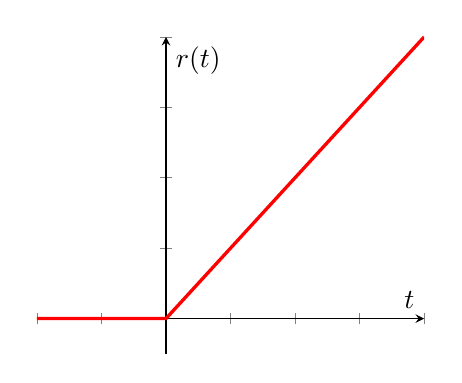
\begin{tikzpicture}
    	\begin{axis}[
            small, axis x line=middle, axis y line=center, xlabel=$t$, ylabel=$r(t)$, xmin=-2, xmax=4, ymin=-0.5, ymax=4,
            xticklabels={,,}, % to hide the numbers on the x axis
            yticklabels={,,} % to hide the numbers on the y axis
            ]
            \addplot+[very thick, red, mark=none, sharp plot] coordinates {(-2,0) (0,0) (4,4)};
    	\end{axis}
    \end{tikzpicture}
	\caption{Représentation de la rampe unitaire $r(t)$}
\end{figure}

\paragraph{\'Echelon unitaire de Heaviside $\Gamma(t)$ :}

\[ \Gamma(t) =
\begin{cases}
    0 & \text{si } t < 0 \\
    1 & \text{sinon}
\end{cases} \]

\begin{figure}[!htbp]
	\centering
    \begin{tikzpicture}
    	\begin{axis}[
            small, axis x line=middle, axis y line=center, xlabel=$t$, ylabel=$\Gamma(t)$, xmin=-3, xmax=3, ymin=-0.2, ymax=2,
            xticklabels={,,}, % to hide the numbers on the x axis
            yticklabels={,,} % to hide the numbers on the y axis
            ]
            \addplot+[very thick, red, mark=none, const plot] coordinates {(-4,0) (0,1) (4,1)};
    	\end{axis}
    \end{tikzpicture}
	\caption{Représentation de l'échelon unitaire de Heaviside $\Gamma(t)$}
\end{figure}

\paragraph{Fonction signe $sgn(t)$ :}

\[ sgn(t) =
\begin{cases}
    1 & \text{si } t > 0 \\
    0 & \text{si } t = 0 \\
    -1 & \text{sinon}
\end{cases} \]

\begin{figure}[!htbp]
	\centering
    \begin{tikzpicture}
    	\begin{axis}[
            small, axis x line=middle, axis y line=center, xlabel=$t$, ylabel=$sgn(t)$, xmin=-4, xmax=4, ymin=-2, ymax=2,
            xticklabels={,,}, % to hide the numbers on the x axis
            yticklabels={,,} % to hide the numbers on the y axis
            ]
            \addplot+[very thick, red, mark=none, sharp plot] coordinates {(-4,-1) (0,-1)};
            \addplot+[very thick, red, mark=none, sharp plot] coordinates {(0,1) (4,1)};
            \addplot+[very thick, red, sharp plot] coordinates {(0,0)};
    	\end{axis}
    \end{tikzpicture}
	\caption{Représentation de la fonction signe $sgn(t)$}
\end{figure}

\paragraph{Fonction fenêtre rectangulaire $rect(t)$ :}

\[ rect(t) =
\begin{cases}
    1 & \text{si } |t| \leq \dfrac{T}{2} \\
    0 & \text{sinon}
\end{cases} \]

\[ rect_{T}(t) = \Gamma(t + \dfrac{T}{2}) - \Gamma(t - \dfrac{T}{2}) \]

Signal utilisé pour observer un signal sur un horizon fini de durée $T$. On dit qu'on applique un fenêtrage rectangulaire sur $s(t)$.

\begin{figure}[!htbp]
	\centering
    \begin{tikzpicture}
        \begin{axis}[
            small, axis x line=middle, axis y line=center, xlabel=$t$, ylabel=$rect(t)$, xmin=-4, xmax=4, ymin=-0.5, ymax=3,
            xticklabels={,,}, % to hide the numbers on the x axis
            yticklabels={,,} % to hide the numbers on the y axis
            ]
            \addplot+[very thick, red, mark=none, const plot] coordinates {(-4,0) (-2,1) (2,0) (4,0)};
        \end{axis}
    \end{tikzpicture}
	\caption{Représentation de la fonction fenêtre rectangulaire $rect(t)$}
\end{figure}

\paragraph{Fonction fenêtre triangulaire $tri(t)$ :}

\[ tri(t) =
\begin{cases}
    1-\dfrac{2}{T}|t| & \text{si } |t| \leq \dfrac{T}{2} \\
    0 & \text{sinon}
\end{cases} \]

\[ tri_{T}(t) = \dfrac{2}{T} r(t + \dfrac{T}{2}) - \dfrac{4}{T} r(t) + \dfrac{2}{T} r(t - \dfrac{T}{2}) \]

\begin{figure}[!htbp]
	\centering
    \begin{tikzpicture}
        \begin{axis}[
            small, axis x line=middle, axis y line=center, xlabel=$t$, ylabel=$tri(t)$, xmin=-4, xmax=4, ymin=-0.5, ymax=3,
            xticklabels={,,}, % to hide the numbers on the x axis
            yticklabels={,,} % to hide the numbers on the y axis
            ]
            \addplot+[very thick, red, mark=none, sharp plot] coordinates {(-4,0) (-2,0) (0,1) (2,0) (4,0)};
        \end{axis}
    \end{tikzpicture}
	\caption{Représentation de la fonction fenêtre triangulaire $tri(t)$}
\end{figure}

\paragraph{Impulsion de Dirac $\delta(t)$ :}

\[ \delta(t) =
\begin{cases}
    1 & \text{si } t = 0 \\
    0 & \text{sinon}
\end{cases} \]

L'impulsion $\delta(t)$ est un opérateur qui extrait la valeur du signal lorsque $t = 0$.

\begin{figure}[!htbp]
	\centering
    \begin{tikzpicture}
        \begin{axis}[
            small, axis x line=middle, axis y line=center, xlabel=$t$, ylabel=$\delta(t)$, xmin=-4, xmax=4, ymin=-0.5, ymax=3,
            xticklabels={,,}, % to hide the numbers on the x axis
            yticklabels={,,} % to hide the numbers on the y axis
            ]
            \addplot+[very thick, red, mark=none, const plot] coordinates {(-4,0) (0,1) (0,0) (4,0)};
        \end{axis}
    \end{tikzpicture}
	\caption{Représentation de l'impulsion de Dirac $\delta(t)$}
\end{figure}

\paragraph{Peigne de Dirac $\dirac_{T}(t)$ :}

\[ \dirac_{T}(t) = \sum_{k=-\infty}^{+\infty} \delta(t - kT) \]

\begin{figure}[!htbp]
	\centering
    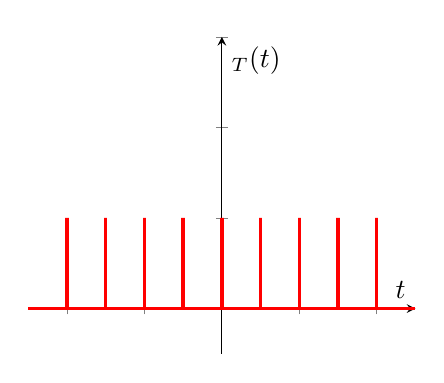
\begin{tikzpicture}
        \begin{axis}[
            small, axis x line=middle, axis y line=center, xlabel=$t$, ylabel=$\dirac_{T}(t)$, xmin=-5, xmax=5, ymin=-0.5, ymax=3,
            xticklabels={,,}, % to hide the numbers on the x axis
            yticklabels={,,} % to hide the numbers on the y axis
            ]
            \addplot+[very thick, red, mark=none, const plot] coordinates {(-5,0) (-4,1) (-4,0) (-3,1) (-3,0) (-2,1) (-2,0) (-1,1) (-1,0) (0,1) (0,0) (1,1) (1,0) (2,1) (2,0) (3,1) (3,0) (4,1) (4,0) (5,0)};
        \end{axis}
    \end{tikzpicture}
	\caption{Représentation du peigne de Dirac $\dirac(t)$}
\end{figure}

\paragraph{Fonction sinus cardinal $sinc(t)$ :}

\[ sinc(t) =
\begin{cases}
    1 & \text{si } t = 0 \\
    \dfrac{sin(\pi t)}{\pi t} & \text{sinon}
\end{cases} \]
\[ sinc(-t) = sinc(t) \]
\[ \forall t = k \in \mathbb{Z}^{*}, sinc(t) = 0 \]

\begin{figure}[!htbp]
	\centering
    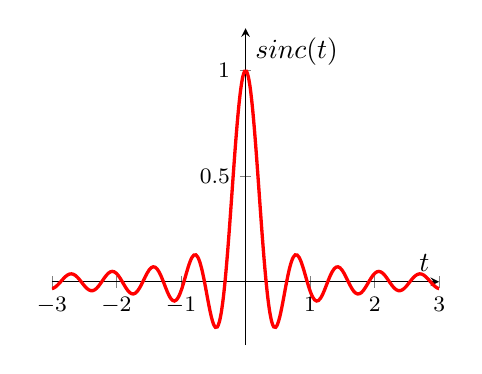
\begin{tikzpicture}
        \begin{axis}[
            small, axis x line=middle, axis y line=center, xlabel=$t$, ylabel=$sinc(t)$, ymin=-0.3, ymax=1.2]
            \addplot+[very thick, red, mark=none, smooth, samples=200, domain=-3:3] {sin(x*180*pi)/(x*pi*pi)};
        \end{axis}
    \end{tikzpicture}
	\caption{Représentation de la fonction sinus cardinal $sinc(t)$}
\end{figure}

\section{Convolution de signaux à temps continu}

Le produit de convolution de deux signaux à temps continu $x(t)$ et $y(t)$ est :
\[ x(t) \otimes y(t) = \int_{-\infty}^{+\infty} x(\nu)y(t-\nu) \mathrm{d}\nu \]

Propriétés : commutativité, associativité, distributivité et élément neutre

\paragraph{Convolution par $\delta(t)$ :}
\[ s(t) \otimes \delta(t-t_{0}) = s(t-t_{0}) \]

\paragraph{Convolution par un peigne de Dirac $\dirac_{T}(t)$ :}
\[ s(t) \otimes \dirac_{T}(t) = \sum_{k=-\infty}^{+\infty} s(t-kT) \]
Convoluer un signal par un peigne de Dirac revient à périodiser le signal à la période T.

\chapter{Analyse des signaux périodiques}

\section{Représentation d'un signal}

Un signal ($s(t) = A \cos(2\pi f_{0}t + \alpha)$) peut être représenté dans un espace à 3 dimensions :
\begin{itemize}
    \item projection sur l'axe du temps $\implies$ une sinusoïde continue
    \item projection sur l'axe des fréquences $\implies$ une raie située en $f = f_{0}$ et de hauteur $A$
\end{itemize}

\section{Les séries de Fourier}

\begin{defi}[Série de Fourier]
    Toute fonction $T$-périodique $s$ peut être décomposée en une somme infinie de fonctions sinusoïdales dont les fréquences sont des multiples de la fréquence fondamentale $f_{0} = \dfrac{1}{T}$.
    \[ s(t) = \dfrac{a_{0}}{2} + \sum_{k=1}^{+\infty} a_{k} \cos(2\pi k f_{0} t) + b_{k} \sin(2\pi k f_{0} t) \]
    \[ \text{avec } \begin{cases}
        \dfrac{a_{0}}{2} & \text{ : valeur moyenne ou composante continue} \\
        a_{k} = \frac{2}{T} \int_ {-T/2}^{T/2} s(t) \cos(2\pi f_{0} kt) \mathrm{d}t & \text{ : coefficient de Fourier en cosinus} \\
        b_{k} = \frac{2}{T} \int_ {-T/2}^{T/2} s(t) \sin(2\pi f_{0} kt) \mathrm{d}t & \text{ : coefficient de Fourier en sinus}
    \end{cases} \]
\end{defi}

\paragraph{Harmonique de rang k du signal :}
\[ h_{k}(t) = a_{k} \cos(2\pi kf_{0}t) + b_{k} \sin(2\pi kf_{0}t) \]

\subsection{Séries de Fourier en cosinus}

En prenant en compte la relation :
\[ A \cos(x) + B \sin(x) = \sqrt{A^2 + B^2} \times \cos(x + \arctan(\dfrac{-B}{A})) \]
le développement en séries de Fourier peut s'écrire :
\[ s(t) = A_0 + \sum_{k=1}^{+\infty} A_k \cos(2\pi kf_0 t + \alpha_k) \]

La représentation spectrale qui lui est associée porte le nom de spectre unilatéral.

\subsection{Séries de Fourier complexes}

Rappel de la relation d'Euler :
\[ \cos(\theta) = \dfrac{e^{i\theta} + e^{-i\theta}}{2} \text{ et } \sin(\theta) = \dfrac{e^{i\theta} - e^{-i\theta}}{2i} \]

On montre que la série de Fourier peut être transformée en une série complexe :
\[ s(t) = \sum_{k = -\infty}^{+\infty} X(ik) e^{i2\pi kf_0 t} \]
avec $X(ik)$ le coefficient complexe de la série de Fourier :
\[ X(ik) = \dfrac{1}{T} \int_{-T/2}^{T/2} s(t) e^{-i2\pi kf_0 t} \mathrm{d}t \]

La représentation spectrale qui lui est associée porte le nom de spectre bilatéral.
\[ X(ik) = \dfrac{a_k - ib_k}{2} \text{ et } X(-ik) = \dfrac{a_k + ib_k}{2} \]
\[ a_k = X(ik) + X(-ik) \text{ et } b_k = i[X(ik) - X(-ik)] \]
\[ \arg(X(ik)) = -arg(X(-ik)) = \alpha_k \]

\paragraph{Dans le cas des spectres bilatéraux :}
\[ ||X(ik)|| = ||X(-ik)|| = \dfrac{A_k}{2} \text{ avec } k\neq0 \]
\[ ||X(0)|| = A_0 \]
\[ ||X(ik)|| = ||\dfrac{a_k - ib_k}{2}|| = \dfrac{\sqrt{a^{2}_{k} + b^{2}_{k}}}{2} = \dfrac{A_k}{2} \]
\[ \arg(X(ik)) = \arctan(\dfrac{-b_k}{a_k}) = \alpha_k = -\arctan(\dfrac{b_k}{a_k}) = -arg(X(ik)) \]

\subsection{Quelques propriétés des séries de Fourier :}
\[ X(ik) = \dfrac{A_k}{2} e^{i\alpha_k} \]
\[ X(-ik) = \dfrac{A_k}{2} e^{-i\alpha_k} \]

\paragraph{Signal pair (s(t) = s(-t)) :}
\[ a_k = \dfrac{4}{T} \int_{0}^{T/2} s(t) \cos(2\pi kf_0 t) \mathrm{d}t \text{ et } b_k = 0 \]

\paragraph{Signal pair (s(t) = s(-t)) :}
\[ a_k = 0 \text{ et } b_k = \dfrac{4}{T} \int_{0}^{T/2} s(t) \sin(2\pi kf_0 t) \mathrm{d}t \]

\textbf{Exemple :}

Soit le signal $s$ : $s(t) =
\begin{cases}
    \frac{\pi}{4} & \text{ si } t \in ] 2n\pi ; (2n+1)\pi [ \\
    \frac{-\pi}{4} & \text{ sinon}
\end{cases}$

$s$ est impair $\implies a_k = 0 \text{ et } b_k = \dfrac{-1}{2k} [cos(kt)]_{0}^{\pi} = \dfrac{1}{2k} \times -cos(kt+1)$

\subsection{Suites d'impulsions}

\subsubsection{Suites d'impulsions rectangulaires}

Impulsions rectangulaires de largeur $2\Delta t$ et de période $T$ :
\[ X(ik) = \dfrac{A\Delta t}{T} \underbrace{\dfrac{\sin(k\pi f_0 \Delta t)}{k\pi f_0 \Delta t}}_{=\mathrm{sinc}(k\pi f_0 \Delta t)} \]

\begin{figure}[!htbp]
	\centering
    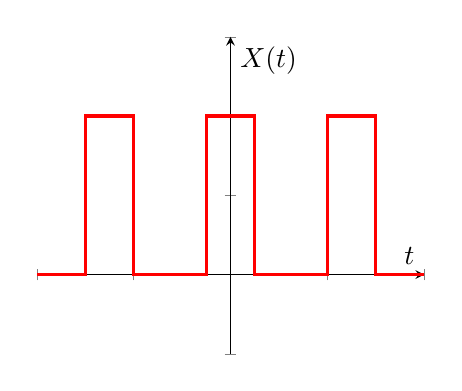
\begin{tikzpicture}
    	\begin{axis}[
            small, axis x line=middle, axis y line=center, xlabel=$t$, ylabel=$X(t)$, xmin=-4, xmax=4, ymin=-0.5, ymax=1.5,
            xticklabels={,,}, % to hide the numbers on the x axis
            yticklabels={,,} % to hide the numbers on the y axis
            ]
            \addplot+[very thick, red, mark=none, const plot] coordinates {(-4,0) (-3,1) (-2,0) (-0.5,1) (0.5,0) (2,1) (3,0) (4,0)};
    	\end{axis}
    \end{tikzpicture}
	\caption{Représentation de la suite d'impulsions rectangulaires}
\end{figure}

\subsubsection{Suites d'impulsions triangulaires}

Impulsions triangulaires de largeur $2\Delta t$ et de période $T$ :
\[ X(ik) = \dfrac{A\Delta t}{T} \mathrm{sinc}^2(k\pi f_0 \Delta t) \]

\begin{figure}[!htbp]
	\centering
    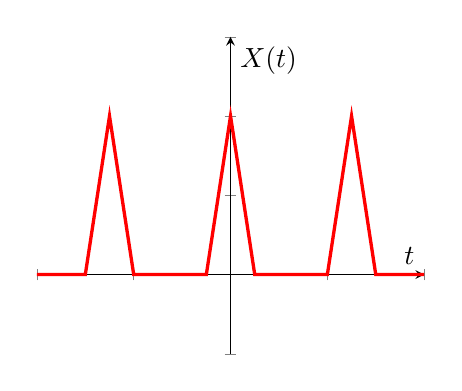
\begin{tikzpicture}
    	\begin{axis}[
            small, axis x line=middle, axis y line=center, xlabel=$t$, ylabel=$X(t)$, xmin=-4, xmax=4, ymin=-0.5, ymax=1.5,
            xticklabels={,,}, % to hide the numbers on the x axis
            yticklabels={,,} % to hide the numbers on the y axis
            ]
            \addplot+[very thick, red, mark=none, sharp plot] coordinates {(-4,0) (-3,0) (-2.5, 1) (-2,0) (-0.5,0) (0,1) (0.5,0) (2,0) (2.5,1) (3,0) (4,0)};
    	\end{axis}
    \end{tikzpicture}
	\caption{Représentation de la suite d'impulsions triangulaires}
\end{figure}

\subsubsection{Suites d'exponentielles décroissantes}

\[ s(t) = \Delta e^{-t/\tau} \text{ avec } \tau \text{ le taux d'amortissement} \]
\[ S(ik) = \dfrac{A}{T} \dfrac{-\tau (e^{-t(\frac{T}{\tau}+i2k\pi f_0 t)})-1}{1+i2\pi kf_0 \tau} \]

 \[ \tau <<< T \implies S(ik) = \dfrac{A\tau}{T} \dfrac{1}{1+i2\pi kf_0 \tau} \]

\subsection{Énergie d'un signal}
\[ E(x) = 1/T \int_{-T/2}^{T/2} s^2(t) \mathrm{d}t \]

\paragraph{Puissance fournie par une harmonique de rang p :}
\[ E_p = \dfrac{1}{T} \int_{-T/2}^{T/2}(a_p \cos(2\pi f_0 pt) + b_p \sin(2\pi f_0 pt)) \mathrm{d}t = \dfrac{a_p^2 + b_p^2}{2} \]

\subsection{Formule de Parseval}

\begin{defi}[Formule de Parseval]
    \[ \dfrac{1}{T} \int_{-T/2}^{T/2} s^2(t) \mathrm{d}t = \dfrac{a_0^2}{4} + \sum_{k=1}^{+\infty} \dfrac{a_k^2 + b_k^2}{2} \]
    \[ \dfrac{1}{T} \int_{-T/2}^{T/2} s^2(t) \mathrm{d}t = A_0^2 + \sum_{k=1}^{+\infty} \dfrac{A_k^2}{2} = \sum_{-\infty}^{+\infty} ||X(ik)||^2 \]
\end{defi}

\subsection{Décalage temporel}

\[ x(t) \longrightarrow y(t) = x(t + t_d) \]
\[ Y(ik) = X(ik) + e^{i2\pi kf_0 t_d} \]
\[ \underbrace{\arg(Y(ik))}_{\beta_k} = \underbrace{\arg(X(ik))}_{\alpha_k} + 2\pi kf_0 t_d \]

\subsection{Modulation d'amplitude}

\[ x(t) = m(t) \times p(t) \]
Si $p(t)$ est sinusoïdale, on peut la remplacer par 2 phaseurs de fréquences $\pm f_p$.
\[ \cos(2\pi kf_pt) = \dfrac{e^{i2\pi kf_pt} + e^{-i2\pi kf_pt}}{2} \]

On montre que :
\[ x(t) = e^{\pm i2\pi f_pt}m(t) \Leftrightarrow X(ik) = M(i(kf_p \pm f_p)) \]

À une multiplication par un phaseur dans le domaine temporel correspond à un décalage dans l'espace de fréquence.

\chapter{Analyse des signaux apériodiques}

\section{Passage de la décomposition en séries de Fourier (DSF) à la transformée de Fourier (TF)}

Le passage d'un signal périodique à un signal apériodique peut se faire en considérant que la période $T$ devient de plus en plus grande pour tendre finalement vers $+\infty$.

\begin{defi}[Signal apériodique]
    Un signal apériodique $x(t)$ peut être défini à l'aide de son intégrale de Fourier
    \[ x(t) = \int_{-\infty}^{+\infty} X(if) e^{i2\pi ft} \mathrm{d}f \]
    \[ X(if) = \int_{-\infty}^{+\infty} x(t) e^{-i2\pi ft} \mathrm{d}t \]

    $X(if)$ est la transformée de Fourier directe de $x(t)$. $x(t)$ est la transformée de Fourier inverse de $X(if)$.
    \[ X(if) = \TF{x(t)} \]
    \[ x(t) = \mathrm{TF}^{-1} \{X(if)\} \]
\end{defi}

La courbe $X(if)$ en fonction de la fréquence f est le spectre du signal x. Si le signal $x(t)$ ne possède pas de symétries particulières, sa densité spectrale d'amplitude est une fonction complexe :
\[ x(t) \xrightarrow{\mathrm{TF}} X(if) = X_r(if) + iX_i(if) \]

La décomposition d'un signal $x(t)$ en ses composantes spectrales ($\TF{x(t)} = X(if)$) à l'aide de la transformée de Fourier porte le nom d'analyse spectrale ou analyse de Fourier.

Inversement, la synthèse d'un signal à l'aide de la transformée de Fourier inverse est la synthèse ou synthèse de Fourier.

\subsection{Propriétés}

\paragraph{Linéarité :}

\[
\begin{rcases}
    x(t) \xrightarrow{\mathrm{TF}} X(if) \\
    y(t) \xrightarrow{\mathrm{TF}} Y(if)
\end{rcases} \implies ax(t) + by(t) \xrightarrow{\mathrm{TF}} aX(if) + bY(if) \text{ avec } (a,b) \in \mathbb{C}^2\]

Donc la transformée de Fourier est une transformation linéaire.

\paragraph{Décalage temporel :}

\[ x(t) \xrightarrow{\mathrm{TF}} X(if) \]
\[ x(t + t_0) \xrightarrow{\mathrm{TF}} X(if) e^{i2\pi ft_0} \]

\subsubsection{Décalage fréquentiel}

\[ x(t) \xrightarrow{\mathrm{TF}} X(if) \]
\[ x(t) e^{i2\pi f_0t} \xrightarrow{\mathrm{TF}} X(i(f-f_p)) \]

\paragraph{Changement d'échelle :}

\[ \TF{ x(at)} = \dfrac{1}{||a||} X(i(\dfrac{f}{a})) \text{ avec } a \neq 0 \]

\paragraph{Parité :}

Si le signal $x$ est pair :
\[ X(if) = 2 \int_{0}^{+\infty} x(t) \cos(2\pi ft) \mathrm{d}t \]

Si le signal $x$ est impair :
\[ X(if) = -2i \int_{0}^{+\infty} x(t) \sin(2\pi ft) \mathrm{d}t \]

\paragraph{Spectre d'une impulsion rectangulaire $\mathrm{rect}_{\Delta t}(t)$ de largeur $\Delta t$ :}

\begin{figure}[!htbp]
	\centering
    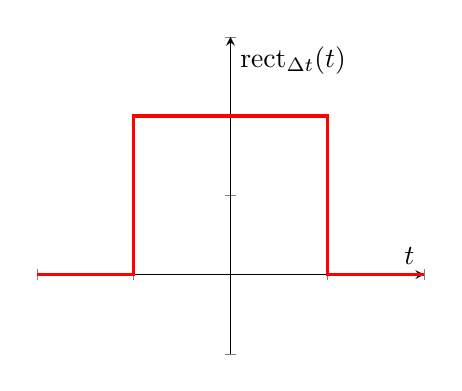
\begin{tikzpicture}
    	\begin{axis}[
            small, axis x line=middle, axis y line=center, xlabel=$t$, ylabel=$\mathrm{rect}_{\Delta t}(t)$, xmin=-4, xmax=4, ymin=-0.5, ymax=1.5,
            xticklabels={,,}, % to hide the numbers on the x axis
            yticklabels={,,} % to hide the numbers on the y axis
            ]
            \addplot+[very thick, red, mark=none, const plot] coordinates {(-4,0) (-2,1) (2,0) (4,0)};
    	\end{axis}
    \end{tikzpicture}
	\caption{Représentation d'une impulsion rectangulaire}
\end{figure}

\[ \mathrm{rect}_{\Delta t}(t) =
\begin{cases}
    A & \text{ si } |t| \leq \dfrac{\Delta t}{2} \\
    0 & \text{ sinon}
\end{cases} \]

Spectre de $\mathrm{rect}_{\Delta t}(t)$ :
\[ \mathrm{RECT}_{\Delta t}(if) = \TF{ \mathrm{rect}_{\Delta t}(t)} \]
\[ = \int_{-\infty}^{+\infty} \mathrm{rect}_{\Delta t}(t) e^{-i2\pi ft} \mathrm{d}t \]
\[ = \int_{-\Delta t / 2}^{\Delta t / 2} A e^{-i2\pi ft} \mathrm{d}t \]
\[ = A[\dfrac{e^{-i2\pi ft}}{-i2\pi f}]_{-\Delta t / 2}^{\Delta t / 2} \]
\[ = \dfrac{A}{\pi f} (\dfrac{e^{i\pi f\Delta t} - e^{-i\pi f\Delta t}}{2i}) \]
\[ = \dfrac{A\Delta t}{\pi f \Delta t} \sin(\pi f\Delta t) \]
\[ = \mathrm{sinc}(\pi f\Delta t) = A\Delta t \times \mathrm{sinc}(\pi f\Delta t) = \TF{ \mathrm{rect}_{\Delta t}(t)} \]

La densité spectrale d'amplitude d'nue impulsion rectangulaire centrée en t=0 est donnée par un sinus cardinal.

\paragraph{Spectre d'un sinus amorti}

\[ y(t) = \begin{cases}
    0 & \text{ si } t < 0 \\
    Ae^{-at} \sin(2\pi f_pt) \text{ si } t \geq 0
\end{cases} \]
\[ Y(if) = A\dfrac{2\pi f_p}{(s + i2\pi f)^2 + (2\pi f_p)^2} \in \mathbb{C} \]

\paragraph{Spectre de deux impulsions}

\begin{figure}[!htbp]
	\centering
    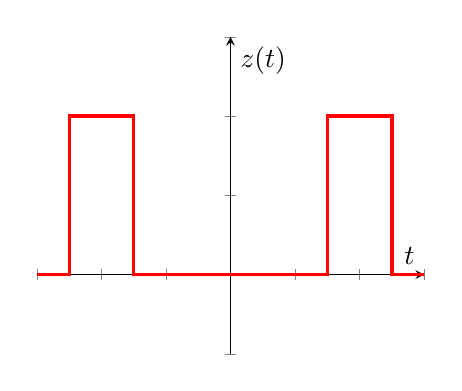
\begin{tikzpicture}
    	\begin{axis}[
            small, axis x line=middle, axis y line=center, xlabel=$t$, ylabel=$z(t)$, xmin=-6, xmax=6, ymin=-0.5, ymax=1.5,
            xticklabels={,,}, % to hide the numbers on the x axis
            yticklabels={,,} % to hide the numbers on the y axis
            ]
            \addplot+[very thick, red, mark=none, const plot] coordinates {(-6,0) (-5,1) (-3, 0) (3,1) (5,0) (6,0)};
    	\end{axis}
    \end{tikzpicture}
	\caption{Représentation de deux impulsions rectangulaires}
\end{figure}

\[ z(t) = \mathrm{rect}_{\Delta t}(t - \dfrac{t_0}{2}) + \mathrm{rect}_{\Delta t}(t + \dfrac{t_0}{2}) \]

Comme la transformée de Fourier est linéaire et $\TF{ x(t + t_0)} = X(if)e^{i2\pi ft_0}$, on a :
\[ Z(if) = 2A\Delta t \times \mathrm{sinc}(\underbrace{\pi f\Delta t)(e^{-i\pi ft_0} + e^{i\pi ft_0}}_{cos(\pi ft_0)}) \]

\paragraph{Spectre de l'exponentielle décroissante :}
\[ x(t) = \begin{cases}
    0 & \text{ si } t < 0 \\
    e^{-at} \text{ si } t \geq 0
\end{cases} \]
\[ X(if) = \dfrac{1}{a+i2\pi f} \]

\paragraph{Spectre de l'exponentielle décroissante symétrique :}
\[ x(t) = e^{-a|t|} \text{ avec } t \in \mathbb{R} \]
\[ X(if) = \dfrac{2a}{a^2+(2\pi f)^2} \]

\paragraph{Spectre du signal unité :}

\begin{figure}[!htbp]
	\centering
    \begin{tikzpicture}
    	\begin{axis}[
            small, axis x line=middle, axis y line=center, xlabel=$t$, ylabel=$z(t)$, xmin=-6, xmax=6, ymin=-0.5, ymax=1.5,
            xticklabels={,,}, % to hide the numbers on the x axis
            yticklabels={,,} % to hide the numbers on the y axis
            ]
            \addplot+[very thick, red, mark=none, const plot] coordinates {(-6,1) (6,1)};
    	\end{axis}
    \end{tikzpicture}
	\caption{Représentation de deux impulsions rectangulaires}
\end{figure}

Le signal $x(t) = 1, \forall t \in \mathbb{R}$ peut être décrit à partir de l'exponentielle décroissante :
\[ x(t) = 1 = \lim_{a \to 0} e^{-a|t|} \text{ avec } t \in \mathbb{R} \]
\[ \TF{ x(t)} = \int_{-\infty}^{+\infty} \lim_{a \to 0} e^{-a|t|} e^{-i2\pi ft} \mathrm{d}t \]
\[ X(if) = \lim_{a \to 0} \dfrac{2a}{a^2 + (2\pi f)^2} = \begin{cases}
    0 & \text{ si } f \neq 0 \\
    +\infty & \text{ si } f = 0
\end{cases} \]

On obtient une impulsion de Dirac :
\[ \TF{ x(t) = 1} = X(if) = \delta(f) \]

\paragraph{Spectre d'un phaseur}

Un phaseur de fréquence $f_0$ peut s'écrire :
\[ x(t) = e^{i2\pi f_0t} = \lim_{a \to 0} e^{-a|t|} e^{i2\pi f_0t} \]

En utilisant :
\[ \begin{cases}
    \TF{ e^{-a|t|} = \dfrac{2a}{a^2 + (2\pi f)^2}} \\
    x(t)e^{i2\pi ft} \xrightarrow{\mathrm{TF}} X(i(f-f_0))
\end{cases} \]

on a :
\[ X(if) = \lim_{a \to 0} \dfrac{2a}{a^2 + (2\pi(f-f_0))^2} \]
\[ = \begin{cases}
    +\infty & \text{ si } f = f_0 \\
    0 & \text{ si } f \neq f_0
\end{cases} \]

Donc la transformée de Fourier d'un phaseur de fréquence $f_0$ est une impulsion de Dirac située en $f=f_0$ :
\[ X(if) = \delta(f-f_0) \]

\paragraph{Spectre d'un signal sinusoïdal :}

Un signal sinusoïdal peut être vu comme la somme de deux phaseurs complexes conjugués.

\[ x(t) = \cos(2\pi f_0 t) = \dfrac{e^{i2\pi f_0t} + e^{-i2\pi f_0t}}{2} \]
\[ \implies X(if) = \TF{ \dfrac{1}{2} e^{i2\pi f_0t} + \dfrac{1}{2} e^{-i2\pi f_0t}} \]
\[ = \dfrac{1}{2} \TF{e^{i2\pi f_0t}} + \dfrac{1}{2} \TF{e^{i2\pi (-f_0)t}} \]
\[ = \dfrac{1}{2} \delta(f-f_0) + \dfrac{1}{2} \delta(f+f_0) \]

\chapter{Numérisation des signaux}

\section{Chaine de traitement de signal}

\begin{center}
    Signal analogique \\
    $\downarrow$ \\
    Acquisition (convertisseur analogique-numérique) \\
    $\downarrow$ \\
    Traitement numérique (calculateur) \\
    $\downarrow$ \\
    Restitution (convertisseur numérique-analogique) \\
    $\downarrow$ \\
    Signal analogique
\end{center}

\section{Échantillonage}

Avant le traitement numérique par un calculateur, un signal doit être représenté par une suite de valeurs numériques prélevées régulièrement (échantillonage).

On obtient la séquence $(x_n)_{n \in \mathbb{Z}}$ avec $x_n = x(nT_e)$.

L'intervalle de temps $T_e$ séparant deux mesures successives est appelé période d'échantillonnage.

\subsection{Analyse temporelle}

\[ x_e(t) = x(t) \times \dirac_{T_e}(t) \]

\subsection{Analyse fréquentielle}

\[ x_e(t) = x(t) \times \dirac_{T_e}(t) = x(t) \sum_{k = -\infty}^{+\infty} \delta(t-kT_e) \]
\[ X_e(if) = \TF{ x_e(t)} = \TF{ x(t)} \otimes \TF{ \dirac_e(t)} \]
\[ X_e(if) = X(if) \otimes \dfrac{1}{T_e} \dirac_{\frac{1}{T_e}}(f) = X(if) \otimes f_e \dirac_{f_e}(f) \]
\[ \text{car } \TF{\dirac_{T_e}(t)} = f_e \dirac_{f_e}(f) \]

Donc le spectre de base $X(if)$ est répété en tous les multiples de la fréquence d'échantillonnage $f_e$.
\[ X_e(if) = X(if) \otimes f_e \dirac_{f_e}(f) = f_e \sum_{k = -\infty}^{+\infty} X(i(f-kf_e)) \]

\begin{figure}[!htbp]
	\centering
    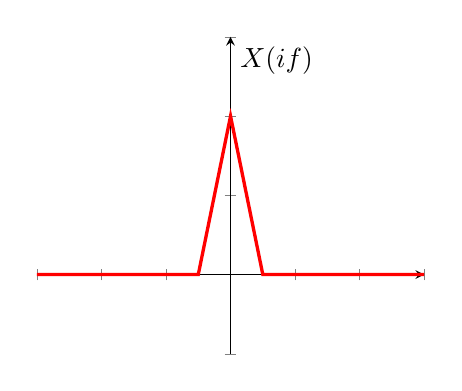
\begin{tikzpicture}
    	\begin{axis}[
            small, axis x line=middle, axis y line=center, ylabel=$X(if)$, xmin=-6, xmax=6, ymin=-0.5, ymax=1.5,
            xticklabels={,,}, % to hide the numbers on the x axis
            yticklabels={,,} % to hide the numbers on the y axis
            ]
            \addplot+[very thick, red, mark=none, sharp plot] coordinates {(-6,0) (-1,0) (0,1) (1,0) (6,0)};
    	\end{axis}
    \end{tikzpicture}
    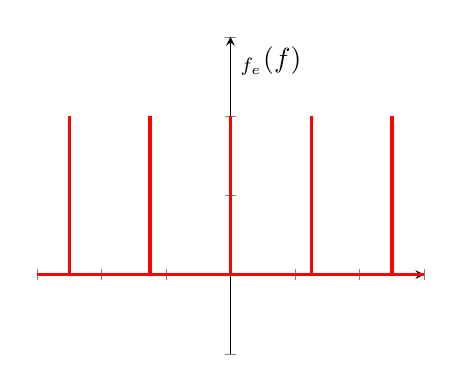
\begin{tikzpicture}
    	\begin{axis}[
            small, axis x line=middle, axis y line=center, ylabel=$\dirac_{f_e}(f)$, xmin=-6, xmax=6, ymin=-0.5, ymax=1.5,
            xticklabels={,,}, % to hide the numbers on the x axis
            yticklabels={,,} % to hide the numbers on the y axis
            ]
            \addplot+[very thick, red, mark=none, const plot] coordinates {(-6,0) (-5,1) (-5,0) (-2.5,1) (-2.5,0) (0,1) (0,0) (2.5,1) (2.5,0) (5,1) (5,0) (6,0)};
    	\end{axis}
    \end{tikzpicture}
    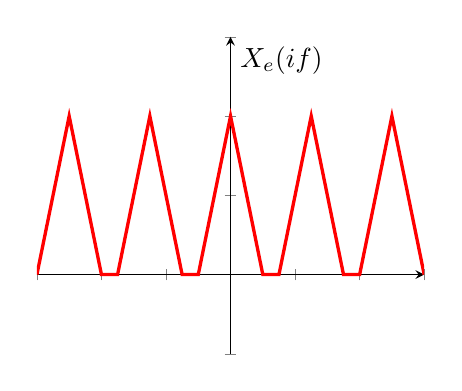
\begin{tikzpicture}
    	\begin{axis}[
            small, axis x line=middle, axis y line=center, ylabel=$X_e(if)$, xmin=-6, xmax=6, ymin=-0.5, ymax=1.5,
            xticklabels={,,}, % to hide the numbers on the x axis
            yticklabels={,,} % to hide the numbers on the y axis
            ]
            \addplot+[very thick, red, mark=none, sharp plot] coordinates {(-6,0) (-5,1) (-4,0) (-3.5,0) (-2.5,1) (-1.5,0) (-1,0) (0,1) (1,0) (1.5,0) (2.5,1) (3.5,0) (4,0) (5,1) (6,0) (6,0)};
    	\end{axis}
    \end{tikzpicture}
	\caption{Représentation de l'analyse fréquentielle}
\end{figure}

\paragraph{Principe}

Répétition du spectre de base autour de $kf_e \implies$ spectres qui vont se superposer si $f_e$ est trop petite. Si on réduit $f_e$, on diminue la distance entre les spectres qui, pour finir, se recouvrent (recouvrement spectral).

\begin{defi}[Théorème d'échantillonnage (ou de Nyquist–Shannon)]
    Un signal x(t) peut être représenté par une suite de valeurs échantillonnées si la fréquence d'échantillonnage $f_e$ est au moins deux fois plus élevée que la plus grande de fréquences contenue dans le signal.
    \[ f_e > 2f_{max} \Leftrightarrow T_e < \dfrac{T_{min}}{2} \]
\end{defi}

\subsection{Types d'échantillonnage}

\subsubsection{Échantillonnage idéal}

Échantillonnage impliquant des impulsions infiniment courtes (n'est pas réalisable physiquement).

\subsubsection{Échantillonnage réel}

La modélisation de l'échantillonnage par $\dirac_{T_e}(t)$ est erronée (impossible d'obtenir des impulsions de durée nulle). Par conséquent, chaque impulsion va avoir une durée très courte $\tau$ donc l'échantillonnage est modélisé par la multiplication de $x(t)$ par une suite d'impulsions rectangulaires de largeur $\tau$ (train d'impulsions).

\subsubsection{Échantillonnage naturel}

Amplitude égale à $x(t)$ pendant la durée $\tau$

\[ \mathrm{tr}(t) = \mathrm{rect}_\tau \otimes \underbrace{\sum_{k=-\infty}^{+\infty} \delta(t-kt_e)}_{\dirac_{T_e}(t)} \]
\[ \mathrm{TR}(f) = [\tau \mathrm{sinc}(\tau \pi f)] \times [f_e \dirac_{f_e}(f)] = \tau f_e \mathrm{sinc}(\tau \pi f) \sum_{k=-\infty}^{+\infty} \delta(f-kf_e) \]

\[ x_e(t) = x(t) \times \mathrm{tr}(t) \]
\[ X_e(if) = X(if) \otimes \mathrm{TR}(if) = X(if) \otimes [\tau f_e \mathrm{sinc}(\tau \pi f) \sum_{k=-\infty}^{+\infty} \delta(f-kf_e)] \]
\[ X_e(if) = X(if) \otimes [\tau f_e \sum_{k=-\infty}^{+\infty} \mathrm{sinc}(\tau \pi kf_e) \delta(f-kf_e)] \]
\[ X_e(if) = \tau f_e \sum_{k=-\infty}^{+\infty} \mathrm{sinc}(\tau \pi kf_e) X(f-kf_e) \]

On retrouve la même allure de spectre modulé en amplitude par un sinus cardinal ; l'échantillonnage provoque une déformation du signal.

Expression du spectre initial :
\[ X_{e_0}(f) = \tau f_e X(if) \xrightarrow{\mathrm{TF}^{}} x_{e_0}(t) = \tau f_e x(t) \]

\subsubsection{Échantillonnage régulier (ou bloqueur)}

Amplitude constante et égale à $x(kT_e)$ pendant la durée $\tau$

\[ x_e(t) = \sum_{k=-\infty}^{+\infty} x(kT_e) \mathrm{rect}_{T_e}((t-kT_e)-\dfrac{T_e}{2}) = x(t) \sum_{k=-\infty}^{+\infty} \mathrm{rect}_{T_e}(t-kT_e-\dfrac{T_e}{2}) \]
\[ x_e(t) = (x(t) \dirac_{T_e}(t)) \otimes \mathrm{rect}_{T_e}(t-\dfrac{T_e}{2}) \]
\[ X_e(if) = [X(if) \otimes f_e \dirac_{f_e}(f)] \times [T_e \mathrm{sinc}(\pi T_e f) e^{-i\pi fT_e}] \]
\[ X_e(if) = \mathrm{sinc}(\pi fT_e) e^{-i\pi fT_e} \sum_{k=-\infty}^{+\infty} X(f-kf_e) \]

Expression du spectre initial :
\[ X_{e_0}(f) = e^{-i\pi fT_e} \mathrm{sinc}(\pi fT_e) X(f) \]

Le spectre $X_e(f)$ n'est pas identique au spectre $X(f)$ puisque son amplitude est modulée par la fonction sinus cardinal. L'échantillonnage régulier introduit une déformation du signal par rapport à l'échantillonnage idéal ou naturel.

\subsubsection{Échantillonnage moyenneur}

Amplitude égale à la moyenne de $x(t)$ sur l'intervalle $\tau$

\[ x_e(kT_e) = \dfrac{1}{\tau} \int_{kT_e - \frac{\tau}{2}}^{kT_e + \frac{\tau}{2}} x(t) \mathrm{d}t \]

En utilisant la fonction fenêtre rectangulaire :
\[ x_e(kT_e) = \dfrac{1}{\tau} \int_{kT_e - \frac{\tau}{2}}^{kT_e + \frac{\tau}{2}} \mathrm{rect}_\tau(t-kT_e) x(t) \mathrm{d}t \]
\[ x_e(kT_e) = \dfrac{1}{\tau} [\mathrm{rect}_\tau(t) \otimes x(t)] \delta(t-kT_e) \]
\[ x_e(t) = \dfrac{1}{\tau} \sum_{k = -\infty}^{+\infty} [\mathrm{rect}_\tau (t) \otimes x(t)] \delta(t-kT_e) \]
\[ x_e(t) = \dfrac{1}{\tau} [\mathrm{rect}_\tau (t) \otimes x(t)] \dirac_{T_e}(t) \]
\[ X_e(f) = \dfrac{1}{\tau} [\tau \mathrm{sinc}(\pi \tau f) X(f)] \otimes f_e \dirac_{f_e}(f) \]
\[ X_e(f) = f_e \sum_{k=-\infty}^{+\infty} \mathrm{sinc}(\pi \tau (f-kf_e)) X(f-kf_e) \]

Expression du spectre initial :
\[ X_{e_0}(f) = f_e \mathrm{sinc}(\pi \tau f) X(f) \]

Extraction d'un signal à partir d'un signal échantillonné (pour obtenir $x(t)$ à partir de $x_e(t)$) :
\[ X_e(f) = f_e \sum_{k=-\infty}^{+\infty} X(f-kf_e) \]

En utilisant un filtre passe-bas idéal de fréquence de coupure $f_c = \dfrac{f_e}{2}$, on peut réaliser l'extraction du signal. La fonction réalisée par le filtre est la fonction fenêtre $\mathrm{rect}_{f_e}(f)$.

\begin{defi}[Théorème de la transformée inverse de la fenêtre rectangulaire]
    \[ \mathrm{TF}^{-1} \{ \mathrm{rect}_{f_e}(f) \} = f_e \mathrm{sinc}(\pi f_e t) \]
\end{defi}

Le spectre de base s'exprimera par :
\[ X_{e_0}(f) = X_e(f) \mathrm{rect}_{f_e}(f) \]
\[ x_{e_0}(t) = x_e(t) \otimes f_e \mathrm{sinc}(\pi f_et) \]
\[ x_{e_0}(t) = x_e(t) \otimes f_e \mathrm{sinc}(\pi f_e t) \]
\[ \text{or } x_e(t) = \sum_{-\infty}^{+\infty} x(kT_e) \delta(t-kT_e) \]
\[ \implies x_{e_0}(t) = f_e (\sum_{-\infty}^{+\infty} x(kT_e) \delta(t-kT_e)) \otimes \mathrm{sinc}(\pi f_e t) \]
\[ x_{e_0}(t) = f_e \sum_{-\infty}^{+\infty} x(kT_e) \mathrm{sinc}(\pi f_e (t=kT_e)) \]
\[ \text{d'autre part } X_{e_0}(f) = f_e X(f) \]
\[ \implies \mathrm{TF}^{-1} \{ X_{e_0}(f) = f_e x(t) \} \]
\[ \implies x_{e_0}(t) = f_e x(t) \]
\[ \implies x(t) = \dfrac{1}{f_e} x_{e_0}(t) \]
\[ x(t) = \sum_{-\infty}^{+\infty} x(kT_e) \mathrm{sinc}(\pi f_e (t-kT_e)) \]

\section{Quantification des signaux}

Quantifier un signal revient à approximer sa valeur par une valeur discrète la plus proche.

\begin{defi}[Le pas de quantification]
    Le convertisseur effectue la numérisation du signal analogique et délivre des séquences codées avec un pas de quantification $Q$ dépendant du nombre de bits de convertisseur.

    \[ Q = \dfrac{\Delta_{\mathrm{CAN}}}{2^n} \]

    \[ \text{avec } \begin{cases}
        \Delta_{\mathrm{CAN}} & \text{ le domaine de conversion du convertisseur} \\
        n & \text{ le nombre de bits}
    \end{cases} \]

    Résolution d'un convertisseur :
    \[ R_\mathrm{CAN} = \dfrac{Q}{\Delta_\mathrm{CAN}} = \dfrac{1}{2^n} \]

    Erreur de quantification :
    \[ E_Q = \dfrac{Q}{2} \]
\end{defi}

\section{Codage des signaux}

Le codage consiste à attribuer à chacun des $2^n$ niveaux issus de la quantification un code binaire sur $n$ bits.

\subsection{Signe de signal constant (codage unipolaire)}

Codage binaire naturel :
\[ N = \sum_{i=0}^{n-1} b_i 2^i = b_0 2^0 + ... + 2^{n-1} b_{n-1} \]
\[ \text{avec } \begin{cases}
    b_{n-1} & \text{ le MSB (Most Significant Bit)} \\
    b_{0} & \text{ le LSB (Least Significant Bit)}
\end{cases} \]

Au code $N$ correspond la tension $Q$.

\subsection{Signe du signal variable (codage bipolaire)}

Code d'amplitude de signe : code qui reprend le code binaire naturel avec en tête un bit de signe.

\section{Transformée de Fourier Discrète (TFD)}

Le calcul de la transformée de Fourier à l'aide d'un calculateur pose des problèmes (temps de calcul, mémoire nécessaire).
\[ \TF{x(t)} = X(f) = \int_{-\infty}^{+\infty} x(t) e^{-i2\pi ft} \d{t} \]

Cela revient à calculer une infinité d'échantillons. Il faut donc discrétiser la fonction temporelle, discrétiser la fonction fréquentielle et tronquer la fonction temporelle.

En approchant l'intégrale par une somme d'aires de rectangles de durée $T_e$ et en limitant la durée d'intégration à l'intervalle $[0, (N-1)T_e]$, on obtient :
\[ X(f) \simeq T_e \sum_{n=0}^{N-1} x(nT_e) e^{-i2\pi fnT_e} \]

On obtient pour les valeurs de fréquence $f_k = \dfrac{kf_e}{n}$ :
\[ X(f) = T_e \sum_{n=0}^{N-1} x(nT_e) e^{-i2\pi \frac{kf_e}{N} nT_e} \]

\begin{defi}[Tranformée de Fourier Discrète (TFD)]
    On appelle tranformée de Fourier discrète d'une suite de $N$ termes $\{ x(0), ..., x(N-1) \}$ la suite de $N$ termes \{ X(0), ..., X(N-1) \} définie par :
    \[ X(k) = \sum_{n=0}^{N-1} x(n) e^{\frac{-i2\pi nk}{N}} \]

    Les $N$ termes $x(n)$ sont les échantillons d'un signal analogique échantillonné $x(n) = x(nT_e) = x_n$ et les $N$ termes $X(k)$ correspondent à une approximation de la transformée de Fourier de ce signa; aux $N$ points de fréquence $f_k = \dfrac{kf_e}{N}$ avec $k \in \{ 0, ..., N-1 \}$ c'est-à-dire $f \in [0, f_e]$.

    Inversion de la tranformée de Fourier discrète :
    \[ x(n) = \dfrac{1}{N} \sum_{k=0}^{N-1}X(k) e^{\frac{i2\pi nk}{N}} \]
\end{defi}

\begin{defi}[Théorème de Parseval]
    \[ \sum_{n=0}^{N-1} ||x(n)||^2 = \dfrac{1}{N} \sum_{n=0}^{N-1} ||x(k)||^2 \]
\end{defi}

\begin{defi}[Transformée de Fourier Rapide (TFR)]
    \[ \mathrm{TFD} \implies X(k) = \sum_{n=0}^{N-1} x(n) e^{\frac{-i2\pi kn}{N}} \]
    \[ \text{soit } \omega = e^{\frac{-i2\pi}{N}} \text{ donc :} \]
    \[ \begin{bmatrix}
        X(0) \\
        X(1) \\
        X(2) \\
        \vdots \\
        X(N-1)
    \end{bmatrix}
    = \begin{bmatrix}
        1 & 1 & 1 & \cdots & 1 \\
        1 & \omega & \omega^2 & \cdots & \omega^{N=-1} \\
        1 & \omega^2 & \omega^4 & \cdots & \omega^{2(N-1)} \\
        \vdots & \vdots & \vdots & \ddots & \vdots \\
        1 & \omega^{N-1} & \omega^{2(N-1)} & \cdots & \omega^{(N-1)(N-1)}
    \end{bmatrix} \begin{bmatrix}
        x(0) \\
        x(1) \\
        x(2) \\
        \vdots \\
        x(N-1)
    \end{bmatrix} \]
    Évaluer ces sommes coûte $N^2$ produits complexes et $N(N-1)$ sommes complexes.

    Pour calculer la transformée de Fourier discrète en temps réel, on dispose d'algorithmes de calcul permettant d'obtenir les résultats beaucoup plus rapidement.

    Ces algorithmes sont connus sous le nom de transformée de Fourier rapide (TFR) ou fast Fourier transform (FFT).

    Le plus connu des algorithmes FFT est celui de Cooley-Tukey qui réduit à $N \log(N)$ le nombre de multiplications complexes.
\end{defi}

\textbf{Applications :}

On comsidère la suite $x(n)$.
\[ x(n) = \begin{cases}
    1 & \text{si } n \in \{ -1, 0, 1 \} \\
    \dfrac{1}{2} & \text{si } n \in \{ -2, 2 \} \\
    0 & \text{si } n \in \{ -m, -(m-1), ..., -4, -3 \} \cup \{ 3, 4, ..., m-1, m \}
\end{cases} \]

\begin{figure}[!htbp]
	\centering
    \begin{tikzpicture}
    	\begin{axis}[
            axis x line=middle, axis y line=center, xmin=-5.5, xmax=5.5, ymin=-0.5, ymax=1.5]
            \addplot [only marks, red] table {
            0 1
            -1 1
            1 1
            -2 .5
            2 .5
            -3 0
            3 0
            -4 0
            4 0
            -5 0
            5 0
            };
    	\end{axis}
    \end{tikzpicture}
\end{figure}

\chapter{Systèmes de traitement de signal}

\section{Transformée de Laplace (TL)}

\begin{defi}[Transformée de Laplace (TL)]
    La tranformée de Laplace d'un signal $x(t)$ est donnée par :
    \[ \TL{x(t)} = X(p) = \int_0^{+\infty} x(t) e^{-pt} \d t \]
    \[ \text{avec } p=i2\pi f \text{ la fréquence complexe} \]
\end{defi}

\subsection{Propriétés de la tranformée de Laplace :}

$x(t) \xrightarrow{\mathrm{TL}} X(p)$

\textbf{Linéarité :} $ax(t) + by(t) \xrightarrow{\mathrm{TL}} aX(p) + bY(p)$

\textbf{Homothétie :} $x(at) \xrightarrow{\mathrm{TL}} \dfrac{1}{|a|} X(\frac{p}{a})$ avec $a \in \mathbb{R}$

\textbf{Translation :} $x(t-a) \xrightarrow{\mathrm{TL}} X(p) e^{-ap}$ avec $a \in \mathbb{R}$

\textbf{Dérivation :} \\
$\frac{\d x(t)}{\d t} \xrightarrow{\mathrm{TL}} pX(p) - x(0)$ \\
$\frac{\d x^2(t)}{\d t^2} \xrightarrow{\mathrm{TL}} p^2X(p) - px(0) - x'(0)$ \\
$\vdots$ \\
$\frac{\d x^n(t)}{\d t^n} \xrightarrow{\mathrm{TL}} p^nX(p) - p^{n-1}x(0) - \dots - p^0 x^{(n-1)}(0)$

\textbf{Intégration :} $\int_0^t x(\tau) \d \tau \xrightarrow{\mathrm{TL}} \dfrac{1}{p} X(p)$

\begin{defi}[Théorème de Borel]
    \[ x(t) \otimes y(t) \xrightarrow{\mathrm{TL}} X(p) Y(p) \]
    \[ x(t) y(t) \xrightarrow{\mathrm{TL}} X(p) \otimes Y(p) \]
\end{defi}

\textbf{Transformée de Laplace d'une fonction $T_0$ périodique :} $x(t) \xrightarrow{\mathrm{TL}} X(p) = \dfrac{1}{1-e^{-pT_0}} \int_0^{T_0} e^{-pt} x(t) \d t$

\begin{defi}[Théorème de la valeur initiale et de la valeur finale]
    \[ x(0) = \lim_{p \to +\infty} pX(p)\]
    \[ \lim_{t \to +\infty} x(t) = \lim_{p \to 0} pX(p) \]
\end{defi}

\section{Systèmes linéaires invariants dans le temps (SLIT)}

\begin{defi}[Systèmes linéaires invariants dans le temps]
    \paragraph{Système :} Structure physique recevant un signal d'entrée $x(t)$ et délivre un signal de sortie $y(t)$. \\
    Si $x(t)$ et $y(t)$ sont analogiques, le système est dit analogique.

    {\Large schéma 1}

    \paragraph{Système invariant dans le temps :} Système dont les caractéristiques de comportement ne se modifient pas dans le temps.

    {\Large schéma 2}
\end{defi}

\subsection{Analyse des systèmes invariants dans le temps}

\textbf{Analyse temporelle :} \\
Observation du comportement en fonction du temps \\
$\implies$ utilisation de fonctions d'excitation (étude de régime transitoire)

\textbf{Analyse fréquentielle :} \\
Observation du comportement en fonction de la variation de la fréquence \\
$\implies$ connaître la réponse du système à une excitation sinusoïdale à différentes fréquences

\subsubsection{Réponse impulsionnelle $h(t)$}

Entrée du système : impulsion de Dirac \\
Sortie du système : $h(t)$

But : apprécier la stabilité du système

Un système linéaire d'entrée $e(t)$ et de réponse impulsionnelle $h(t)$ a pour sortie s(t) tel que :
\[ s(t) = e(t) \otimes h(t) = \int_{-\infty}^{+\infty} e(r) h(t - r) \d r\]

{\Large schéma 3}

\subsubsection{Réponse indicielle $d_i(t)$}

Entrée du système : échelon unité $\Gamma (t)$ \\
Sortie du système : $d_i(t)$

But : observer l'évolution vers un régime permanent de la sortie suite à une discontinuité du signal d'entrée

\[ d_i(t) = \int_0^t h(r) \d r \]

{\Large schéma 4}

\subsubsection{Réponse à une rampe $r(t)$}

\[ r(t) = at \xrightarrow{\mathrm{TL}} \dfrac{a}{p^2} \]

But : utilisé à l'entrée des systèmes qui ne peuvent pas subir de varations trop brusques

{\Large schéma 5}

\textbf{Lien avec la réponse impulsionnelle :}
\[ \dfrac{\d^2 r(t)}{\d t^2} = h(t) \]

\textbf{Lien avec la réponse indicielle :}
\[ r(t) = \int_0^t d_i(\tau) \d \tau \]

\subsubsection{Réponse fréquentielle}

Réponse à une entrée sinusoïdale

$H(j\omega)$ : transmittance isochrone ou FT

\subsubsection{Fonction de transfert}

C'est la tranformée de Laplace de la réponse impulsionnelle :
$H(p) = \dfrac{Y(p)}{X(p)}$ avec $Y(p) = \TL{y(t)}$ et $X(p) = \TL{x(t)}$

On a $p = i2\pi f = i\omega$ \\
$H(p) = H(i\omega)$

\textbf{Détermination isochrone de la FT équivalente :} \\

En série :
{\Large schéma 6}

En paralèle :
{\Large schéma 7}

Lien avec la réponse indicielle $d_i(t)$ :
\[ d_i(t) = \mathrm{TL}^{-1}\{ \frac{H(p)}{p} \} \]

\subsubsection{Diagramme de Bode}

Moyen de représenter le comportement fréquentiel d'un système

Deux tracés :
\begin{itemize}
    \item Gain en décibel (dB) : $G_{dB} = 20 \log (|| H(j\omega) ||)$
    \item Phase en degré : $arg(H(j\omega))$
\end{itemize}

L'échelle de pulsations est logarithmique et est exprimée en $rad/s$.

{\Large schéma 8}

\subsection{Stabilité des systèmes}

Un système est stable au sens EBSB (Entrée Bornée Sortie Bornée) si tout signal d'entrée borné produit un signal de sortie borné c'est-à-dire que la réponse impulsionnelle est absolument intégrable.
\[ \int_{-\infty}^{+\infty} ||h(t)|| \d t = ||h||_1 < +\infty \]

\textbf{Lien avec la réponse impulsionnelle $h(t)$ :}
\begin{itemize}
    \item si $h(t) \to 0$, le système est asymptotiquement stable
    \item si $h(t)$ est borné sans tendre vers $0$, le système est stable
    \item si $h(t)$ diverge, le système est instable
\end{itemize}

\end{document}
